\documentclass[11pt,a4paper]{article}
\usepackage[
    left=0.73in,
    right=0.73in,
    top=.8in,
    bottom=.50in,
    paperheight=11in,
    paperwidth=8.5in
]{geometry}

\usepackage{array}
\newcolumntype{C}[1]{>{\centering\let\newline\\\arraybackslash\hspace{0pt}}m{#1}}
\usepackage{graphicx}
\usepackage{float} % Used with H specifier for floats

\begin{document}
% Cover Page
\pagenumbering{gobble}
\begin{center}
\textbf{
    \Large{ECE 543: Introduction to Digital Systems}
    \\~\\
    \large{Instructor: Bessam Zuhair Al Jewad, Ph.D.}
    \\[1.25in]
    \LARGE{Prelab \#4: Fault Detection in Digital Logic}
    \\[0.62in]
    \large{Prepared for Himadri Basu (TA)\\~\\By Christopher Chin}
    \\[1.25in]
    \LARGE{Section 6}
    \\[1.25in]
    \Large{Department of Electrical and Computer Engineering\\
           University of New Hampshire}
    \\[1.25in]
    \Large{\today}
}
\end{center}
\clearpage
\pagenumbering{arabic}

% TOC
\tableofcontents
\pagebreak

% Pages
\section{Introduction}
The objective of this experiment is to detect common errors and faults in actual logic systems.
We will implement an XS-3 to BCD converter.
BCD is binary encoded decimal, a number system in base 2.
0010 is $2_{10}$. 0011 is $3_{10}$. 0100 is $4_{10}$
XS-3 is a number system where the lowest value (0) represents negative three.
Subsequent digits follow a binary system: $-2_{10}$ is 0001 and $0_{10}$ is 0011.

\section{Equipment Required}
\begin{itemize}
    \item Global Specialties Design and Prototyping PB-505
    \item Wire leads
    \item 7400 TTL Integrated Circuit (4)
    \item Logic Probe (1)
\end{itemize}
\section{Procedure}
\subsection{BCD to XS-3 conversion}
To convert from BCD to XS-3: add $011_2$ to the BCD value.

\begin{tabular}{| C{1.7cm} | C{1.7cm} |}
    \hline BCD  & XS-3 \\
    \hline 0000 & 0011 \\
    \hline 0001 & 0100 \\
    \hline 0010 & 0101 \\
    \hline 0011 & 0110 \\
    \hline 0100 & 0111 \\
    \hline 0101 & 1000 \\
    \hline 0110 & 1001 \\
    \hline 0111 & 1010 \\
    \hline 1000 & 1011 \\
    \hline 1001 & 1100 \\
    \hline 1010 & 1101 \\
    \hline 1011 & 1110 \\
    \hline 1100 & 1111 \\
    \hline
\end{tabular}
\subsection{XS-3 to BCD conversion}
To convert from XS-3 to BCD: subtract $011_2$ to the XS-3 value.

\begin{tabular}{| C{1.7cm} | C{1.7cm} |}
    \hline BCD  & XS-3 \\
    \hline 0000 & 0011 \\
    \hline 0001 & 0100 \\
    \hline 0010 & 0101 \\
    \hline 0011 & 0110 \\
    \hline 0100 & 0111 \\
    \hline 0101 & 1000 \\
    \hline 0110 & 1001 \\
    \hline 0111 & 1010 \\
    \hline 1000 & 1011 \\
    \hline 1001 & 1100 \\
    \hline 1010 & 1101 \\
    \hline 1011 & 1110 \\
    \hline 1100 & 1111 \\
    \hline
\end{tabular}
\subsection{K-map}
XS-3: ABCD where A is most significant bit

\begin{tabular}{| C{1.7cm} | C{1.7cm} | C{1.7cm} | C{1.7cm} | C{1.7cm} |}
    \hline A  & 00 & 01 & 11 & 10 \\
    \hline 00 & 0 & 0 & 0 & 0 \\
    \hline 01 & 0 & 1 & 1 & 1 \\
    \hline 11 & 1 & ~ & ~ & ~ \\
    \hline 10 & 1 & 1 & 1 & 1 \\
    \hline
\end{tabular}

\begin{tabular}{| C{1.7cm} | C{1.7cm} | C{1.7cm} | C{1.7cm} | C{1.7cm} |}
    \hline B  & 00 & 01 & 11 & 10 \\
    \hline 00 & 0 & 1 & 1 & 1 \\
    \hline 01 & 1 & 0 & 0 & 0 \\
    \hline 11 & 1 & ~ & ~ & ~ \\
    \hline 10 & 0 & 1 & 1 & 1 \\
    \hline
\end{tabular}

\begin{tabular}{| C{1.7cm} | C{1.7cm} | C{1.7cm} | C{1.7cm} | C{1.7cm} |}
    \hline C  & 00 & 01 & 11 & 10 \\
    \hline 00 & 1 & 0 & 1 & 0 \\
    \hline 01 & 1 & 0 & 1 & 0 \\
    \hline 11 & 1 & ~ & ~ & ~ \\
    \hline 10 & 1 & 0 & 0 & 0 \\
    \hline
\end{tabular}

\begin{tabular}{| C{1.7cm} | C{1.7cm} | C{1.7cm} | C{1.7cm} | C{1.7cm} |}
    \hline D  & 00 & 01 & 11 & 10 \\
    \hline 00 & 1 & 0 & 0 & 1 \\
    \hline 01 & 1 & 0 & 0 & 1 \\
    \hline 11 & 1 & ~ & ~ & ~ \\
    \hline 10 & 1 & 0 & 0 & 1 \\
    \hline
\end{tabular}
\subsection{Boolean expression of the proposed K map}
A: $S_3'S_2 + S_3S_2S_1'S_0' + S_3S_2$

B: $S_3'S_2' + S_2S_1'S_0' + S_3S_2'$

C: $S_1'S_0' + S_2S_1S_0$

D: $S_1'S_0' + S_1S_0'$
\subsection{Gate Diagram}
\begin{figure}[H]
    \centering
    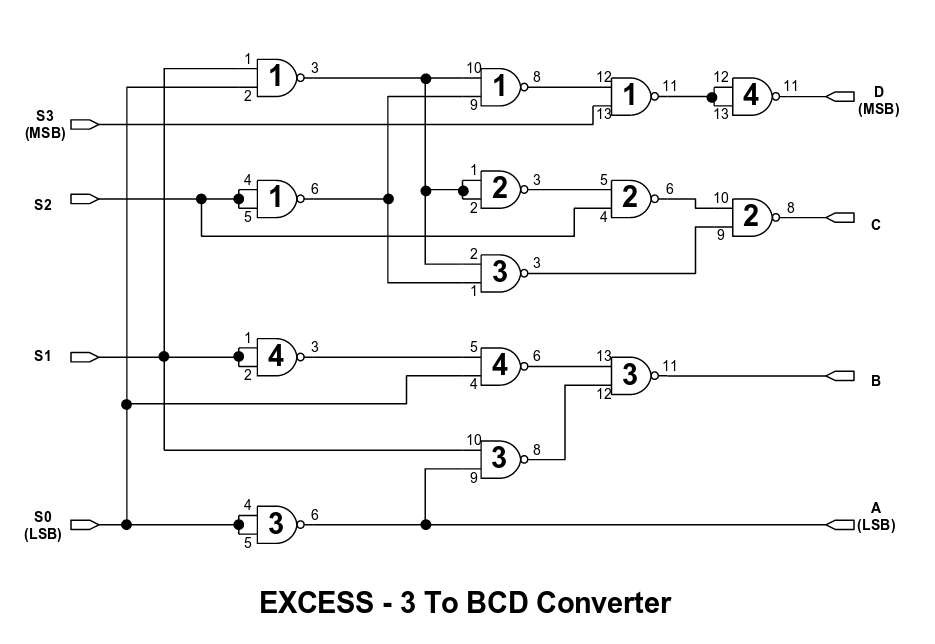
\includegraphics[width=7in]{XS3-BCD.png}
    \caption{XS-3 to BCD Wiring Diagram}
\end{figure}
\subsection{Circuit Diagram}
\begin{figure}[H]
    \centering
    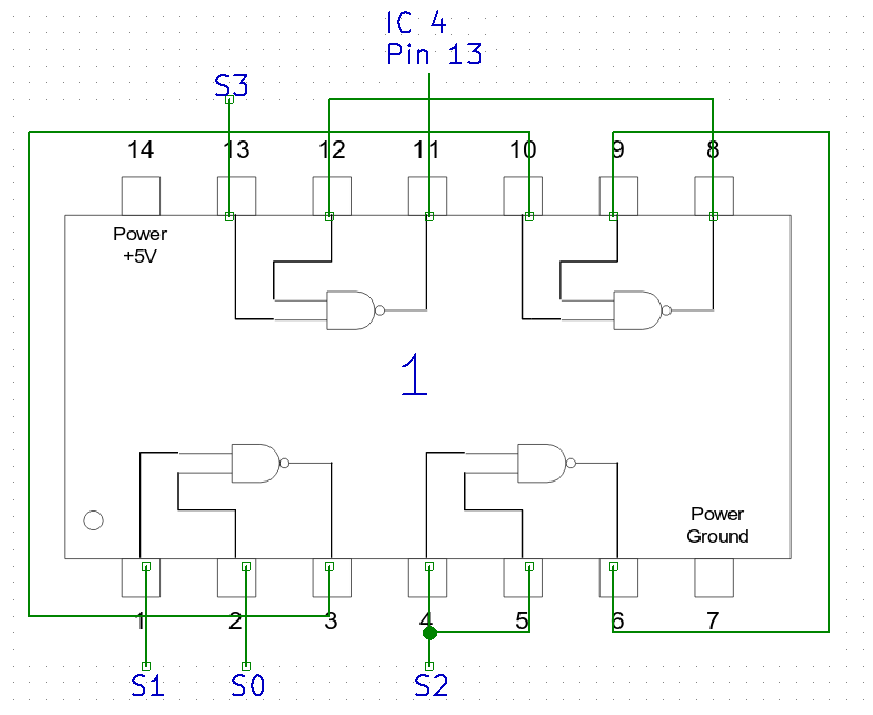
\includegraphics[width=5in]{IC1.png}
    \caption{IC1 Wiring Diagram}
\end{figure}
\begin{figure}[H]
    \centering
    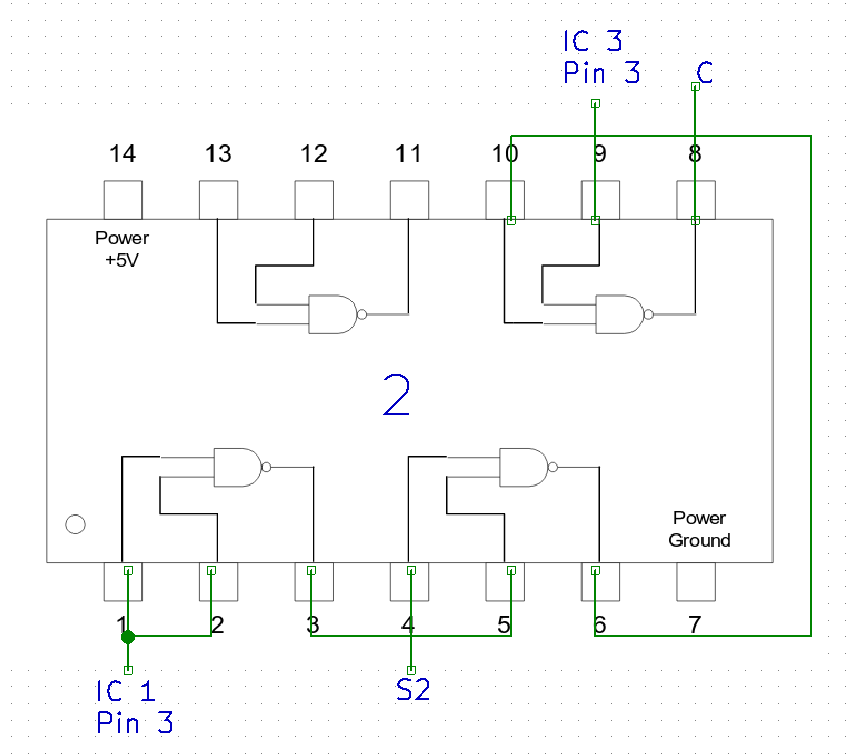
\includegraphics[width=5in]{IC2.png}
    \caption{IC2 Wiring Diagram}
\end{figure}
\begin{figure}[H]
    \centering
    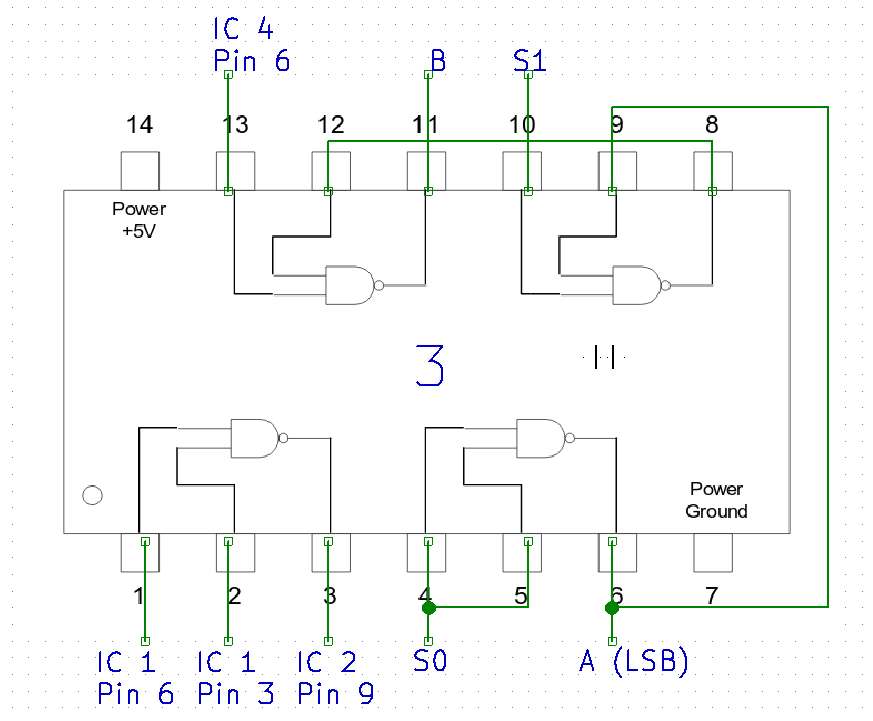
\includegraphics[width=5in]{IC3.png}
    \caption{IC3 Wiring Diagram}
\end{figure}
\begin{figure}[H]
    \centering
    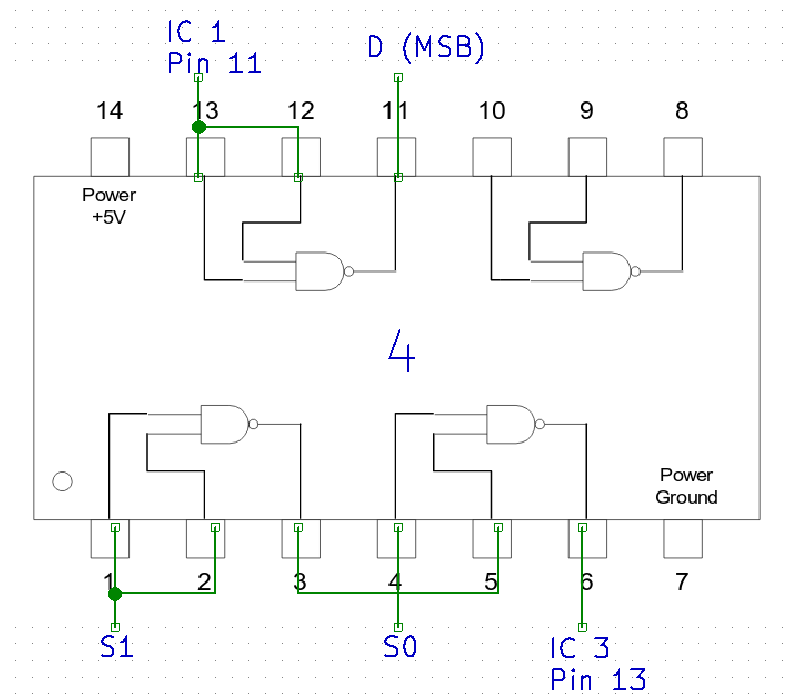
\includegraphics[width=5in]{IC4.png}
    \caption{IC4 Wiring Diagram}
\end{figure}
\subsection{Seven Segment Display}
The seven segment display contains two digits. Each digit has a set of pins 5 holes horizontally
and 4 holes vertically. The rows of these pins are connected. The four rows represent a digit
in a BCD value with the first row being the most significant bit.
\section{Truth Table}
\begin{enumerate}
    \item IC 1 \\
        \begin{tabular}{| C{1.55cm} | C{1.55cm} | C{1.55cm} | C{1.55cm} | C{1.55cm} | C{1.55cm} | C{1.55cm} | C{1.55cm} |}
            \hline
                \multicolumn{4}{|c|}{Inputs} &
                \multicolumn{3}{|c|}{Intermediates} &
                Output \\
            \hline S0 & S1 & S2 & S3 & Pin 3 & Pin 6 & Pin 8 & IC4 Pin13 \\
            \hline 0 & 0 & 0 & 0 & 1 & 1 & 0 & 1\\
            \hline 1 & 0 & 0 & 0 & 1 & 1 & 0 & 1\\
            \hline 0 & 1 & 0 & 0 & 1 & 1 & 0 & 1\\
            \hline 1 & 1 & 0 & 0 & 0 & 1 & 1 & 1\\
            \hline 0 & 0 & 1 & 0 & 1 & 0 & 1 & 1\\
            \hline 1 & 0 & 1 & 0 & 1 & 0 & 1 & 1\\
            \hline 0 & 1 & 1 & 0 & 1 & 0 & 1 & 1\\
            \hline 1 & 1 & 1 & 0 & 0 & 0 & 1 & 1\\
            \hline 0 & 0 & 0 & 1 & 1 & 1 & 0 & 1\\
            \hline 1 & 0 & 0 & 1 & 1 & 1 & 0 & 1\\
            \hline 0 & 1 & 0 & 1 & 1 & 1 & 0 & 1\\
            \hline 1 & 1 & 0 & 1 & 0 & 1 & 1 & 0\\
            \hline 0 & 0 & 1 & 1 & 1 & 0 & 0 & 1\\
            \hline 1 & 0 & 1 & 1 & 1 & 0 & 0 & 1\\
            \hline 0 & 1 & 1 & 1 & 1 & 0 & 0 & 1\\
            \hline 1 & 1 & 1 & 1 & 0 & 0 & 1 & 0\\
            \hline
        \end{tabular}
    \item IC 2 \\
        \begin{tabular}{| C{1.7cm} | C{1.7cm} | C{1.7cm} | C{1.7cm} | C{1.7cm} | C{1.7cm} |}
            \hline
                \multicolumn{3}{|c|}{Inputs} &
                \multicolumn{2}{|c|}{Intermediates} &
                Output \\
            \hline IC1 Pin3 & S2 & IC3 Pin3 & Pin 3 & Pin 6 & C \\
            \hline 0 & 0 & 0 & 0 & 1 & 1 \\
            \hline 1 & 0 & 0 & 1 & 1 & 1 \\
            \hline 0 & 1 & 0 & 0 & 1 & 1 \\
            \hline 1 & 1 & 0 & 1 & 0 & 1 \\
            \hline 0 & 0 & 1 & 0 & 1 & 0 \\
            \hline 1 & 0 & 1 & 1 & 1 & 0 \\
            \hline 0 & 1 & 1 & 0 & 1 & 0 \\
            \hline 1 & 1 & 1 & 1 & 0 & 1 \\
            \hline
        \end{tabular}
    \item IC 3 \\
        \begin{tabular}{| C{1.2cm} | C{1.2cm} | C{1.2cm} | C{1.2cm} | C{1.2cm} | C{1.2cm} | C{1.2cm} | C{1.2cm} | C{1.2cm} | C{1.2cm} |}
            \hline
                \multicolumn{5}{|c|}{Inputs} &
                \multicolumn{2}{|c|}{Intermediates} &
                \multicolumn{3}{|c|}{Outputs} \\
            \hline IC1 Pin6 & IC1 Pin3 & S0 & S1 & IC4 Pin6 & Pin 6 & Pin 8 & IC2 Pin9 & A & B \\
            \hline 0 & 0 & 0 & 0 & 0 & 1 & 1 & 1 & 1 & 1 \\
            \hline 1 & 0 & 0 & 0 & 0 & 1 & 1 & 1 & 1 & 1 \\
            \hline 0 & 1 & 0 & 0 & 0 & 1 & 1 & 1 & 1 & 1 \\
            \hline 1 & 1 & 0 & 0 & 0 & 1 & 1 & 0 & 1 & 1 \\
            \hline 0 & 0 & 1 & 0 & 0 & 0 & 1 & 1 & 0 & 1 \\
            \hline 1 & 1 & 1 & 0 & 0 & 0 & 1 & 1 & 0 & 1 \\
            \hline 0 & 1 & 1 & 0 & 0 & 0 & 1 & 1 & 0 & 1 \\
            \hline 1 & 0 & 1 & 0 & 0 & 0 & 1 & 0 & 0 & 1 \\
            \hline 0 & 1 & 0 & 1 & 0 & 1 & 0 & 1 & 1 & 1 \\
            \hline 1 & 1 & 0 & 1 & 0 & 1 & 0 & 1 & 1 & 1 \\
            \hline 0 & 0 & 0 & 1 & 0 & 1 & 0 & 1 & 1 & 1 \\
            \hline 1 & 1 & 0 & 1 & 0 & 1 & 0 & 0 & 1 & 1 \\
            \hline 0 & 1 & 1 & 1 & 0 & 0 & 1 & 1 & 0 & 1 \\
            \hline 1 & 0 & 1 & 1 & 0 & 0 & 1 & 1 & 0 & 1 \\
            \hline 0 & 1 & 1 & 1 & 0 & 0 & 1 & 1 & 0 & 1 \\
            \hline 1 & 1 & 1 & 1 & 0 & 0 & 1 & 0 & 0 & 1 \\
            \hline 0 & 0 & 0 & 0 & 1 & 1 & 1 & 1 & 1 & 0 \\
            \hline 1 & 0 & 0 & 0 & 1 & 1 & 1 & 1 & 1 & 0 \\
            \hline 0 & 1 & 0 & 0 & 1 & 1 & 1 & 1 & 1 & 0 \\
            \hline 1 & 1 & 0 & 0 & 1 & 1 & 1 & 0 & 1 & 0 \\
            \hline 0 & 0 & 1 & 0 & 1 & 0 & 1 & 1 & 0 & 0 \\
            \hline 1 & 1 & 1 & 0 & 1 & 0 & 1 & 1 & 0 & 0 \\
            \hline 0 & 1 & 1 & 0 & 1 & 0 & 1 & 1 & 0 & 0 \\
            \hline 1 & 0 & 1 & 0 & 1 & 0 & 1 & 0 & 0 & 0 \\
            \hline 0 & 1 & 0 & 1 & 1 & 1 & 0 & 1 & 1 & 1 \\
            \hline 1 & 1 & 0 & 1 & 1 & 1 & 0 & 1 & 1 & 1 \\
            \hline 0 & 0 & 0 & 1 & 1 & 1 & 0 & 1 & 1 & 1 \\
            \hline 1 & 1 & 0 & 1 & 1 & 1 & 0 & 0 & 1 & 1 \\
            \hline 0 & 1 & 1 & 1 & 1 & 0 & 1 & 1 & 0 & 0 \\
            \hline 1 & 0 & 1 & 1 & 1 & 0 & 1 & 1 & 0 & 0 \\
            \hline 0 & 1 & 1 & 1 & 1 & 0 & 1 & 1 & 0 & 0 \\
            \hline 1 & 1 & 1 & 1 & 1 & 0 & 1 & 0 & 0 & 0 \\
            \hline
        \end{tabular}
    \item IC 4 \\
        \begin{tabular}{| C{1.7cm} | C{1.7cm} | C{1.7cm} | C{1.7cm} | C{1.7cm} | C{1.7cm} |}
            \hline
                \multicolumn{3}{|c|}{Inputs} &
                Intermediate &
                \multicolumn{2}{|c|}{Outputs} \\
            \hline S1 & S0 & IC1 Pin11 & Pin 3 & IC3 Pin13 & D \\
            \hline 0 & 0 & 0 & 1 & 1 & 1 \\
            \hline 1 & 0 & 0 & 0 & 1 & 1 \\
            \hline 0 & 1 & 0 & 1 & 0 & 1 \\
            \hline 1 & 1 & 0 & 0 & 1 & 1 \\
            \hline 0 & 0 & 1 & 1 & 1 & 0 \\
            \hline 1 & 0 & 1 & 0 & 1 & 0 \\
            \hline 0 & 1 & 1 & 1 & 0 & 0 \\
            \hline 1 & 1 & 1 & 0 & 1 & 0 \\
            \hline
        \end{tabular}
\end{enumerate}

\pagebreak
\section{References}
Ronald J. Tocci et al. 2011. Digital Systems: Principles and Applications, 11\textsuperscript{th} Ed.

\end{document}
